\documentclass[1p]{elsarticle_modified}
%\bibliographystyle{elsarticle-num}

%\usepackage[colorlinks]{hyperref}
%\usepackage{abbrmath_seonhwa} %\Abb, \Ascr, \Acal ,\Abf, \Afrak
\usepackage{amsfonts}
\usepackage{amssymb}
\usepackage{amsmath}
\usepackage{amsthm}
\usepackage{scalefnt}
\usepackage{amsbsy}
\usepackage{kotex}
\usepackage{caption}
\usepackage{subfig}
\usepackage{color}
\usepackage{graphicx}
\usepackage{xcolor} %% white, black, red, green, blue, cyan, magenta, yellow
\usepackage{float}
\usepackage{setspace}
\usepackage{hyperref}

\usepackage{tikz}
\usetikzlibrary{arrows}

\usepackage{multirow}
\usepackage{array} % fixed length table
\usepackage{hhline}

%%%%%%%%%%%%%%%%%%%%%
\makeatletter
\renewcommand*\env@matrix[1][\arraystretch]{%
	\edef\arraystretch{#1}%
	\hskip -\arraycolsep
	\let\@ifnextchar\new@ifnextchar
	\array{*\c@MaxMatrixCols c}}
\makeatother %https://tex.stackexchange.com/questions/14071/how-can-i-increase-the-line-spacing-in-a-matrix
%%%%%%%%%%%%%%%

\usepackage[normalem]{ulem}

\newcommand{\msout}[1]{\ifmmode\text{\sout{\ensuremath{#1}}}\else\sout{#1}\fi}
%SOURCE: \msout is \stkout macro in https://tex.stackexchange.com/questions/20609/strikeout-in-math-mode

\newcommand{\cancel}[1]{
	\ifmmode
	{\color{red}\msout{#1}}
	\else
	{\color{red}\sout{#1}}
	\fi
}

\newcommand{\add}[1]{
	{\color{blue}\uwave{#1}}
}

\newcommand{\replace}[2]{
	\ifmmode
	{\color{red}\msout{#1}}{\color{blue}\uwave{#2}}
	\else
	{\color{red}\sout{#1}}{\color{blue}\uwave{#2}}
	\fi
}

\newcommand{\Sol}{\mathcal{S}} %segment
\newcommand{\D}{D} %diagram
\newcommand{\A}{\mathcal{A}} %arc


%%%%%%%%%%%%%%%%%%%%%%%%%%%%%5 test

\def\sl{\operatorname{\textup{SL}}(2,\Cbb)}
\def\psl{\operatorname{\textup{PSL}}(2,\Cbb)}
\def\quan{\mkern 1mu \triangleright \mkern 1mu}

\theoremstyle{definition}
\newtheorem{thm}{Theorem}[section]
\newtheorem{prop}[thm]{Proposition}
\newtheorem{lem}[thm]{Lemma}
\newtheorem{ques}[thm]{Question}
\newtheorem{cor}[thm]{Corollary}
\newtheorem{defn}[thm]{Definition}
\newtheorem{exam}[thm]{Example}
\newtheorem{rmk}[thm]{Remark}
\newtheorem{alg}[thm]{Algorithm}

\newcommand{\I}{\sqrt{-1}}
\begin{document}

%\begin{frontmatter}
%
%\title{Boundary parabolic representations of knots up to 8 crossings}
%
%%% Group authors per affiliation:
%\author{Yunhi Cho} 
%\address{Department of Mathematics, University of Seoul, Seoul, Korea}
%\ead{yhcho@uos.ac.kr}
%
%
%\author{Seonhwa Kim} %\fnref{s_kim}}
%\address{Center for Geometry and Physics, Institute for Basic Science, Pohang, 37673, Korea}
%\ead{ryeona17@ibs.re.kr}
%
%\author{Hyuk Kim}
%\address{Department of Mathematical Sciences, Seoul National University, Seoul 08826, Korea}
%\ead{hyukkim@snu.ac.kr}
%
%\author{Seokbeom Yoon}
%\address{Department of Mathematical Sciences, Seoul National University, Seoul, 08826,  Korea}
%\ead{sbyoon15@snu.ac.kr}
%
%\begin{abstract}
%We find all boundary parabolic representation of knots up to 8 crossings.
%
%\end{abstract}
%\begin{keyword}
%    \MSC[2010] 57M25 
%\end{keyword}
%
%\end{frontmatter}

%\linenumbers
%\tableofcontents
%
\newcommand\colored[1]{\textcolor{white}{\rule[-0.35ex]{0.8em}{1.4ex}}\kern-0.8em\color{red} #1}%
%\newcommand\colored[1]{\textcolor{white}{ #1}\kern-2.17ex	\textcolor{white}{ #1}\kern-1.81ex	\textcolor{white}{ #1}\kern-2.15ex\color{red}#1	}

{\Large $\underline{12a_{0630}~(K12a_{0630})}$}

\setlength{\tabcolsep}{10pt}
\renewcommand{\arraystretch}{1.6}
\vspace{1cm}\begin{tabular}{m{100pt}>{\centering\arraybackslash}m{274pt}}
\multirow{5}{120pt}{
	\centering
	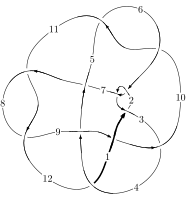
\includegraphics[width=112pt]{../../../GIT/diagram.site/Diagrams/png/1431_12a_0630.png}\\
\ \ \ A knot diagram\footnotemark}&
\allowdisplaybreaks
\textbf{Linearized knot diagam} \\
\cline{2-2}
 &
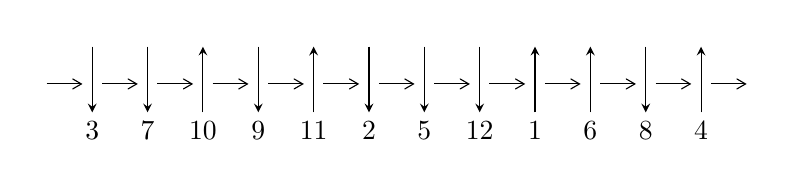
\begin{tikzpicture}[x=20pt, y=17pt]
	% nodes
	\node (C0) at (0, 0) {};
	\node (C1) at (1, 0) {};
	\node (C1U) at (1, +1) {};
	\node (C1D) at (1, -1) {3};

	\node (C2) at (2, 0) {};
	\node (C2U) at (2, +1) {};
	\node (C2D) at (2, -1) {7};

	\node (C3) at (3, 0) {};
	\node (C3U) at (3, +1) {};
	\node (C3D) at (3, -1) {10};

	\node (C4) at (4, 0) {};
	\node (C4U) at (4, +1) {};
	\node (C4D) at (4, -1) {9};

	\node (C5) at (5, 0) {};
	\node (C5U) at (5, +1) {};
	\node (C5D) at (5, -1) {11};

	\node (C6) at (6, 0) {};
	\node (C6U) at (6, +1) {};
	\node (C6D) at (6, -1) {2};

	\node (C7) at (7, 0) {};
	\node (C7U) at (7, +1) {};
	\node (C7D) at (7, -1) {5};

	\node (C8) at (8, 0) {};
	\node (C8U) at (8, +1) {};
	\node (C8D) at (8, -1) {12};

	\node (C9) at (9, 0) {};
	\node (C9U) at (9, +1) {};
	\node (C9D) at (9, -1) {1};

	\node (C10) at (10, 0) {};
	\node (C10U) at (10, +1) {};
	\node (C10D) at (10, -1) {6};

	\node (C11) at (11, 0) {};
	\node (C11U) at (11, +1) {};
	\node (C11D) at (11, -1) {8};

	\node (C12) at (12, 0) {};
	\node (C12U) at (12, +1) {};
	\node (C12D) at (12, -1) {4};
	\node (C13) at (13, 0) {};

	% arrows
	\draw[->,>={angle 60}]
	(C0) edge (C1) (C1) edge (C2) (C2) edge (C3) (C3) edge (C4) (C4) edge (C5) (C5) edge (C6) (C6) edge (C7) (C7) edge (C8) (C8) edge (C9) (C9) edge (C10) (C10) edge (C11) (C11) edge (C12) (C12) edge (C13) ;	\draw[->,>=stealth]
	(C1U) edge (C1D) (C2U) edge (C2D) (C3D) edge (C3U) (C4U) edge (C4D) (C5D) edge (C5U) (C6U) edge (C6D) (C7U) edge (C7D) (C8U) edge (C8D) (C9D) edge (C9U) (C10D) edge (C10U) (C11U) edge (C11D) (C12D) edge (C12U) ;
	\end{tikzpicture} \\
\hhline{~~} \\& 
\textbf{Solving Sequence} \\ \cline{2-2} 
 &
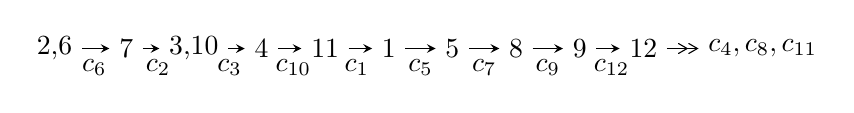
\begin{tikzpicture}[x=23pt, y=7pt]
	% node
	\node (A0) at (-1/8, 0) {2,6};
	\node (A1) at (1, 0) {7};
	\node (A2) at (33/16, 0) {3,10};
	\node (A3) at (25/8, 0) {4};
	\node (A4) at (33/8, 0) {11};
	\node (A5) at (41/8, 0) {1};
	\node (A6) at (49/8, 0) {5};
	\node (A7) at (57/8, 0) {8};
	\node (A8) at (65/8, 0) {9};
	\node (A9) at (73/8, 0) {12};
	\node (C1) at (1/2, -1) {$c_{6}$};
	\node (C2) at (3/2, -1) {$c_{2}$};
	\node (C3) at (21/8, -1) {$c_{3}$};
	\node (C4) at (29/8, -1) {$c_{10}$};
	\node (C5) at (37/8, -1) {$c_{1}$};
	\node (C6) at (45/8, -1) {$c_{5}$};
	\node (C7) at (53/8, -1) {$c_{7}$};
	\node (C8) at (61/8, -1) {$c_{9}$};
	\node (C9) at (69/8, -1) {$c_{12}$};
	\node (A10) at (11, 0) {$c_{4},c_{8},c_{11}$};

	% edge
	\draw[->,>=stealth]	
	(A0) edge (A1) (A1) edge (A2) (A2) edge (A3) (A3) edge (A4) (A4) edge (A5) (A5) edge (A6) (A6) edge (A7) (A7) edge (A8) (A8) edge (A9) ;
	\draw[->>,>={angle 60}]	
	(A9) edge (A10);
\end{tikzpicture} \\ 

\end{tabular} \\

\footnotetext{
The image of knot diagram is generated by the software ``\textbf{Draw programme}" developed by Andrew Bartholomew(\url{http://www.layer8.co.uk/maths/draw/index.htm\#Running-draw}), where we modified some parts for our purpose(\url{https://github.com/CATsTAILs/LinksPainter}).
}\phantom \\ \newline 
\centering \textbf{Ideals for irreducible components\footnotemark of $X_{\text{par}}$} 
 
\begin{align*}
I^u_{1}&=\langle 
-5.91340\times10^{369} u^{144}+1.16876\times10^{370} u^{143}+\cdots+1.70448\times10^{369} b+2.22815\times10^{371},\\
\phantom{I^u_{1}}&\phantom{= \langle  }-3.70382\times10^{371} u^{144}+5.34656\times10^{371} u^{143}+\cdots+7.32926\times10^{370} a+3.08617\times10^{373},\\
\phantom{I^u_{1}}&\phantom{= \langle  }u^{145}- u^{144}+\cdots+111 u+43\rangle \\
I^u_{2}&=\langle 
-47244 u^{25}+102 u^{24}+\cdots+21943 b-77421,\\
\phantom{I^u_{2}}&\phantom{= \langle  }2102618 u^{25}-1405135 u^{24}+\cdots+416917 a+2687295,\;u^{26}-5 u^{24}+\cdots+3 u+1\rangle \\
\\
\end{align*}
\raggedright * 2 irreducible components of $\dim_{\mathbb{C}}=0$, with total 171 representations.\\
\footnotetext{All coefficients of polynomials are rational numbers. But the coefficients are sometimes approximated in decimal forms when there is not enough margin.}
\newpage
\renewcommand{\arraystretch}{1}
\centering \section*{I. $I^u_{1}= \langle -5.91\times10^{369} u^{144}+1.17\times10^{370} u^{143}+\cdots+1.70\times10^{369} b+2.23\times10^{371},\;-3.70\times10^{371} u^{144}+5.35\times10^{371} u^{143}+\cdots+7.33\times10^{370} a+3.09\times10^{373},\;u^{145}- u^{144}+\cdots+111 u+43 \rangle$}
\flushleft \textbf{(i) Arc colorings}\\
\begin{tabular}{m{7pt} m{180pt} m{7pt} m{180pt} }
\flushright $a_{2}=$&$\begin{pmatrix}0\\u\end{pmatrix}$ \\
\flushright $a_{6}=$&$\begin{pmatrix}1\\0\end{pmatrix}$ \\
\flushright $a_{7}=$&$\begin{pmatrix}1\\u^2\end{pmatrix}$ \\
\flushright $a_{3}=$&$\begin{pmatrix}- u\\- u^3+u\end{pmatrix}$ \\
\flushright $a_{10}=$&$\begin{pmatrix}5.05348 u^{144}-7.29482 u^{143}+\cdots-1529.59 u-421.075\\3.46933 u^{144}-6.85702 u^{143}+\cdots-527.016 u-130.724\end{pmatrix}$ \\
\flushright $a_{4}=$&$\begin{pmatrix}13.2152 u^{144}-5.82712 u^{143}+\cdots-2009.43 u-616.681\\4.92450 u^{144}-2.88311 u^{143}+\cdots-622.147 u-167.645\end{pmatrix}$ \\
\flushright $a_{11}=$&$\begin{pmatrix}8.52281 u^{144}-14.1518 u^{143}+\cdots-2056.61 u-551.799\\3.46933 u^{144}-6.85702 u^{143}+\cdots-527.016 u-130.724\end{pmatrix}$ \\
\flushright $a_{1}=$&$\begin{pmatrix}u^3\\u^5- u^3+u\end{pmatrix}$ \\
\flushright $a_{5}=$&$\begin{pmatrix}3.01580 u^{144}-1.99190 u^{143}+\cdots-880.199 u-302.431\\2.54787 u^{144}-4.15288 u^{143}+\cdots-58.9951 u-14.8841\end{pmatrix}$ \\
\flushright $a_{8}=$&$\begin{pmatrix}5.82435 u^{144}-14.4755 u^{143}+\cdots-3307.07 u-852.613\\1.30197 u^{144}-7.24708 u^{143}+\cdots-799.748 u-136.273\end{pmatrix}$ \\
\flushright $a_{9}=$&$\begin{pmatrix}7.02548 u^{144}-13.0533 u^{143}+\cdots-1664.35 u-451.446\\3.09963 u^{144}-6.81289 u^{143}+\cdots-527.426 u-116.601\end{pmatrix}$ \\
\flushright $a_{12}=$&$\begin{pmatrix}-3.17000 u^{144}+10.4896 u^{143}+\cdots+3245.66 u+880.087\\-1.49962 u^{144}+8.59243 u^{143}+\cdots+904.608 u+193.456\end{pmatrix}$\\&\end{tabular}
\flushleft \textbf{(ii) Obstruction class $= -1$}\\~\\
\flushleft \textbf{(iii) Cusp Shapes $= -1.69384 u^{144}+23.7737 u^{143}+\cdots+1298.05 u+121.085$}\\~\\
\newpage\renewcommand{\arraystretch}{1}
\flushleft \textbf{(iv) u-Polynomials at the component}\newline \\
\begin{tabular}{m{50pt}|m{274pt}}
Crossings & \hspace{64pt}u-Polynomials at each crossing \\
\hline $$\begin{aligned}c_{1}\end{aligned}$$&$\begin{aligned}
&u^{145}+59 u^{144}+\cdots-292549 u+1849
\end{aligned}$\\
\hline $$\begin{aligned}c_{2},c_{6}\end{aligned}$$&$\begin{aligned}
&u^{145}- u^{144}+\cdots+111 u+43
\end{aligned}$\\
\hline $$\begin{aligned}c_{3}\end{aligned}$$&$\begin{aligned}
&u^{145}+6 u^{143}+\cdots-200298 u+49447
\end{aligned}$\\
\hline $$\begin{aligned}c_{4}\end{aligned}$$&$\begin{aligned}
&u^{145}-2 u^{144}+\cdots+13 u-1
\end{aligned}$\\
\hline $$\begin{aligned}c_{5},c_{10}\end{aligned}$$&$\begin{aligned}
&u^{145}-3 u^{144}+\cdots+85723 u+9799
\end{aligned}$\\
\hline $$\begin{aligned}c_{7}\end{aligned}$$&$\begin{aligned}
&u^{145}-11 u^{144}+\cdots-3598960 u+268027
\end{aligned}$\\
\hline $$\begin{aligned}c_{8},c_{11}\end{aligned}$$&$\begin{aligned}
&u^{145}- u^{144}+\cdots-6 u-1
\end{aligned}$\\
\hline $$\begin{aligned}c_{9}\end{aligned}$$&$\begin{aligned}
&u^{145}+u^{144}+\cdots-1852 u-8809
\end{aligned}$\\
\hline $$\begin{aligned}c_{12}\end{aligned}$$&$\begin{aligned}
&u^{145}+12 u^{144}+\cdots+14475 u+983
\end{aligned}$\\
\hline
\end{tabular}\\~\\
\newpage\renewcommand{\arraystretch}{1}
\flushleft \textbf{(v) Riley Polynomials at the component}\newline \\
\begin{tabular}{m{50pt}|m{274pt}}
Crossings & \hspace{64pt}Riley Polynomials at each crossing \\
\hline $$\begin{aligned}c_{1}\end{aligned}$$&$\begin{aligned}
&y^{145}+45 y^{144}+\cdots+56069800047 y-3418801
\end{aligned}$\\
\hline $$\begin{aligned}c_{2},c_{6}\end{aligned}$$&$\begin{aligned}
&y^{145}-59 y^{144}+\cdots-292549 y-1849
\end{aligned}$\\
\hline $$\begin{aligned}c_{3}\end{aligned}$$&$\begin{aligned}
&y^{145}+12 y^{144}+\cdots+12484646126 y-2445005809
\end{aligned}$\\
\hline $$\begin{aligned}c_{4}\end{aligned}$$&$\begin{aligned}
&y^{145}-2 y^{144}+\cdots-995 y-1
\end{aligned}$\\
\hline $$\begin{aligned}c_{5},c_{10}\end{aligned}$$&$\begin{aligned}
&y^{145}+117 y^{144}+\cdots-14395117115 y-96020401
\end{aligned}$\\
\hline $$\begin{aligned}c_{7}\end{aligned}$$&$\begin{aligned}
&y^{145}-47 y^{144}+\cdots+2169230447548 y-71838472729
\end{aligned}$\\
\hline $$\begin{aligned}c_{8},c_{11}\end{aligned}$$&$\begin{aligned}
&y^{145}-111 y^{144}+\cdots+244 y-1
\end{aligned}$\\
\hline $$\begin{aligned}c_{9}\end{aligned}$$&$\begin{aligned}
&y^{145}-37 y^{144}+\cdots+6073711804 y-77598481
\end{aligned}$\\
\hline $$\begin{aligned}c_{12}\end{aligned}$$&$\begin{aligned}
&y^{145}+30 y^{144}+\cdots-94703045 y-966289
\end{aligned}$\\
\hline
\end{tabular}\\~\\
\newpage\flushleft \textbf{(vi) Complex Volumes and Cusp Shapes}
$$\begin{array}{c|c|c}  
\text{Solutions to }I^u_{1}& \I (\text{vol} + \sqrt{-1}CS) & \text{Cusp shape}\\
 \hline 
\begin{aligned}
u &= \phantom{-}0.877303 + 0.468272 I \\
a &= \phantom{-}1.57356 - 0.62205 I \\
b &= \phantom{-}0.29748 + 2.26551 I\end{aligned}
 & -2.78991 - 1.90964 I & \phantom{-0.000000 } 0 \\ \hline\begin{aligned}
u &= \phantom{-}0.877303 - 0.468272 I \\
a &= \phantom{-}1.57356 + 0.62205 I \\
b &= \phantom{-}0.29748 - 2.26551 I\end{aligned}
 & -2.78991 + 1.90964 I & \phantom{-0.000000 } 0 \\ \hline\begin{aligned}
u &= \phantom{-}0.882422 + 0.437768 I \\
a &= -0.321281 - 1.299260 I \\
b &= -0.06255 - 1.51339 I\end{aligned}
 & -8.61145 - 1.79826 I & \phantom{-0.000000 } 0 \\ \hline\begin{aligned}
u &= \phantom{-}0.882422 - 0.437768 I \\
a &= -0.321281 + 1.299260 I \\
b &= -0.06255 + 1.51339 I\end{aligned}
 & -8.61145 + 1.79826 I & \phantom{-0.000000 } 0 \\ \hline\begin{aligned}
u &= -0.815077 + 0.543750 I \\
a &= \phantom{-}1.70139 + 2.08254 I \\
b &= \phantom{-}0.93293 - 2.67151 I\end{aligned}
 & -3.68834 + 2.23519 I & \phantom{-0.000000 } 0 \\ \hline\begin{aligned}
u &= -0.815077 - 0.543750 I \\
a &= \phantom{-}1.70139 - 2.08254 I \\
b &= \phantom{-}0.93293 + 2.67151 I\end{aligned}
 & -3.68834 - 2.23519 I & \phantom{-0.000000 } 0 \\ \hline\begin{aligned}
u &= \phantom{-}0.876196 + 0.413458 I \\
a &= \phantom{-}2.72185 + 1.43346 I \\
b &= \phantom{-}0.122814 + 1.077590 I\end{aligned}
 & -4.68823 + 4.69132 I & \phantom{-0.000000 } 0 \\ \hline\begin{aligned}
u &= \phantom{-}0.876196 - 0.413458 I \\
a &= \phantom{-}2.72185 - 1.43346 I \\
b &= \phantom{-}0.122814 - 1.077590 I\end{aligned}
 & -4.68823 - 4.69132 I & \phantom{-0.000000 } 0 \\ \hline\begin{aligned}
u &= -0.590696 + 0.766056 I \\
a &= -1.44442 + 0.92272 I \\
b &= \phantom{-}1.169960 - 0.141258 I\end{aligned}
 & \phantom{-}0.27031 - 7.86888 I & \phantom{-0.000000 } 0 \\ \hline\begin{aligned}
u &= -0.590696 - 0.766056 I \\
a &= -1.44442 - 0.92272 I \\
b &= \phantom{-}1.169960 + 0.141258 I\end{aligned}
 & \phantom{-}0.27031 + 7.86888 I & \phantom{-0.000000 } 0\\
 \hline 
 \end{array}$$\newpage$$\begin{array}{c|c|c}  
\text{Solutions to }I^u_{1}& \I (\text{vol} + \sqrt{-1}CS) & \text{Cusp shape}\\
 \hline 
\begin{aligned}
u &= \phantom{-}0.956142 + 0.395396 I \\
a &= -1.136230 - 0.527024 I \\
b &= -0.094603 + 0.660999 I\end{aligned}
 & -4.86760 - 7.94659 I & \phantom{-0.000000 } 0 \\ \hline\begin{aligned}
u &= \phantom{-}0.956142 - 0.395396 I \\
a &= -1.136230 + 0.527024 I \\
b &= -0.094603 - 0.660999 I\end{aligned}
 & -4.86760 + 7.94659 I & \phantom{-0.000000 } 0 \\ \hline\begin{aligned}
u &= -0.599491 + 0.756559 I \\
a &= \phantom{-}1.33554 - 0.64310 I \\
b &= -0.896372 - 0.235830 I\end{aligned}
 & \phantom{-}4.15674 - 3.15991 I & \phantom{-0.000000 } 0 \\ \hline\begin{aligned}
u &= -0.599491 - 0.756559 I \\
a &= \phantom{-}1.33554 + 0.64310 I \\
b &= -0.896372 + 0.235830 I\end{aligned}
 & \phantom{-}4.15674 + 3.15991 I & \phantom{-0.000000 } 0 \\ \hline\begin{aligned}
u &= -0.390521 + 0.882567 I \\
a &= -0.594345 + 0.451423 I \\
b &= \phantom{-}0.382837 - 1.274910 I\end{aligned}
 & -1.26071 - 5.33735 I & \phantom{-0.000000 } 0 \\ \hline\begin{aligned}
u &= -0.390521 - 0.882567 I \\
a &= -0.594345 - 0.451423 I \\
b &= \phantom{-}0.382837 + 1.274910 I\end{aligned}
 & -1.26071 + 5.33735 I & \phantom{-0.000000 } 0 \\ \hline\begin{aligned}
u &= -0.801456 + 0.537667 I \\
a &= -0.017933 + 0.502510 I \\
b &= -0.325610 + 0.795147 I\end{aligned}
 & -1.55077 + 2.17680 I & \phantom{-0.000000 } 0 \\ \hline\begin{aligned}
u &= -0.801456 - 0.537667 I \\
a &= -0.017933 - 0.502510 I \\
b &= -0.325610 - 0.795147 I\end{aligned}
 & -1.55077 - 2.17680 I & \phantom{-0.000000 } 0 \\ \hline\begin{aligned}
u &= \phantom{-}0.901498 + 0.511632 I \\
a &= -1.07717 - 2.46541 I \\
b &= \phantom{-}2.53524 + 0.74110 I\end{aligned}
 & -3.05457 - 1.67010 I & \phantom{-0.000000 } 0 \\ \hline\begin{aligned}
u &= \phantom{-}0.901498 - 0.511632 I \\
a &= -1.07717 + 2.46541 I \\
b &= \phantom{-}2.53524 - 0.74110 I\end{aligned}
 & -3.05457 + 1.67010 I & \phantom{-0.000000 } 0\\
 \hline 
 \end{array}$$\newpage$$\begin{array}{c|c|c}  
\text{Solutions to }I^u_{1}& \I (\text{vol} + \sqrt{-1}CS) & \text{Cusp shape}\\
 \hline 
\begin{aligned}
u &= -0.533541 + 0.797556 I \\
a &= \phantom{-}0.71732 - 1.34689 I \\
b &= -0.58770 + 1.36493 I\end{aligned}
 & -5.88372 - 4.52346 I & \phantom{-0.000000 } 0 \\ \hline\begin{aligned}
u &= -0.533541 - 0.797556 I \\
a &= \phantom{-}0.71732 + 1.34689 I \\
b &= -0.58770 - 1.36493 I\end{aligned}
 & -5.88372 + 4.52346 I & \phantom{-0.000000 } 0 \\ \hline\begin{aligned}
u &= \phantom{-}0.583401 + 0.758857 I \\
a &= -1.145310 - 0.283574 I \\
b &= \phantom{-}0.791925 - 0.009498 I\end{aligned}
 & \phantom{-}2.68264 + 1.06220 I & \phantom{-0.000000 } 0 \\ \hline\begin{aligned}
u &= \phantom{-}0.583401 - 0.758857 I \\
a &= -1.145310 + 0.283574 I \\
b &= \phantom{-}0.791925 + 0.009498 I\end{aligned}
 & \phantom{-}2.68264 - 1.06220 I & \phantom{-0.000000 } 0 \\ \hline\begin{aligned}
u &= -0.888534 + 0.337951 I \\
a &= \phantom{-}0.211272 - 0.432260 I \\
b &= -0.634572 + 0.402280 I\end{aligned}
 & -1.54724 + 0.94745 I & \phantom{-0.000000 } 0 \\ \hline\begin{aligned}
u &= -0.888534 - 0.337951 I \\
a &= \phantom{-}0.211272 + 0.432260 I \\
b &= -0.634572 - 0.402280 I\end{aligned}
 & -1.54724 - 0.94745 I & \phantom{-0.000000 } 0 \\ \hline\begin{aligned}
u &= -0.537246 + 0.778939 I \\
a &= -1.014390 - 0.014558 I \\
b &= \phantom{-}0.447040 + 0.853657 I\end{aligned}
 & -0.02802 + 2.03103 I & \phantom{-0.000000 } 0 \\ \hline\begin{aligned}
u &= -0.537246 - 0.778939 I \\
a &= -1.014390 + 0.014558 I \\
b &= \phantom{-}0.447040 - 0.853657 I\end{aligned}
 & -0.02802 - 2.03103 I & \phantom{-0.000000 } 0 \\ \hline\begin{aligned}
u &= \phantom{-}0.850709 + 0.409603 I \\
a &= -2.41313 - 0.98350 I \\
b &= \phantom{-}0.195250 - 0.907862 I\end{aligned}
 & -0.162571 + 1.035960 I & \phantom{-0.000000 } 0 \\ \hline\begin{aligned}
u &= \phantom{-}0.850709 - 0.409603 I \\
a &= -2.41313 + 0.98350 I \\
b &= \phantom{-}0.195250 + 0.907862 I\end{aligned}
 & -0.162571 - 1.035960 I & \phantom{-0.000000 } 0\\
 \hline 
 \end{array}$$\newpage$$\begin{array}{c|c|c}  
\text{Solutions to }I^u_{1}& \I (\text{vol} + \sqrt{-1}CS) & \text{Cusp shape}\\
 \hline 
\begin{aligned}
u &= \phantom{-}0.823610 + 0.459896 I \\
a &= \phantom{-}2.48932 + 1.20710 I \\
b &= -1.45968 + 1.21878 I\end{aligned}
 & -2.72559 - 2.32796 I & \phantom{-0.000000 } 0 \\ \hline\begin{aligned}
u &= \phantom{-}0.823610 - 0.459896 I \\
a &= \phantom{-}2.48932 - 1.20710 I \\
b &= -1.45968 - 1.21878 I\end{aligned}
 & -2.72559 + 2.32796 I & \phantom{-0.000000 } 0 \\ \hline\begin{aligned}
u &= -0.923681 + 0.516547 I \\
a &= -0.971498 + 0.142711 I \\
b &= -0.160473 + 1.223340 I\end{aligned}
 & -1.81144 + 1.97771 I & \phantom{-0.000000 } 0 \\ \hline\begin{aligned}
u &= -0.923681 - 0.516547 I \\
a &= -0.971498 - 0.142711 I \\
b &= -0.160473 - 1.223340 I\end{aligned}
 & -1.81144 - 1.97771 I & \phantom{-0.000000 } 0 \\ \hline\begin{aligned}
u &= \phantom{-}0.920288 + 0.193098 I \\
a &= \phantom{-}1.68632 + 0.01894 I \\
b &= -0.142587 - 0.330023 I\end{aligned}
 & -4.69016 - 1.86889 I & \phantom{-0.000000 } 0 \\ \hline\begin{aligned}
u &= \phantom{-}0.920288 - 0.193098 I \\
a &= \phantom{-}1.68632 - 0.01894 I \\
b &= -0.142587 + 0.330023 I\end{aligned}
 & -4.69016 + 1.86889 I & \phantom{-0.000000 } 0 \\ \hline\begin{aligned}
u &= -0.933790 + 0.502928 I \\
a &= -1.92033 + 0.14167 I \\
b &= \phantom{-}0.74017 + 1.36721 I\end{aligned}
 & -2.36535 + 2.64438 I & \phantom{-0.000000 } 0 \\ \hline\begin{aligned}
u &= -0.933790 - 0.502928 I \\
a &= -1.92033 - 0.14167 I \\
b &= \phantom{-}0.74017 - 1.36721 I\end{aligned}
 & -2.36535 - 2.64438 I & \phantom{-0.000000 } 0 \\ \hline\begin{aligned}
u &= -0.752593 + 0.555151 I \\
a &= \phantom{-}1.27984 - 0.77388 I \\
b &= -0.508967 + 1.178150 I\end{aligned}
 & -3.18084 - 4.82889 I & \phantom{-0.000000 } 0 \\ \hline\begin{aligned}
u &= -0.752593 - 0.555151 I \\
a &= \phantom{-}1.27984 + 0.77388 I \\
b &= -0.508967 - 1.178150 I\end{aligned}
 & -3.18084 + 4.82889 I & \phantom{-0.000000 } 0\\
 \hline 
 \end{array}$$\newpage$$\begin{array}{c|c|c}  
\text{Solutions to }I^u_{1}& \I (\text{vol} + \sqrt{-1}CS) & \text{Cusp shape}\\
 \hline 
\begin{aligned}
u &= \phantom{-}0.962052 + 0.472393 I \\
a &= \phantom{-}0.947301 + 0.777991 I \\
b &= -0.562454 - 0.445089 I\end{aligned}
 & -0.68104 - 4.52796 I & \phantom{-0.000000 } 0 \\ \hline\begin{aligned}
u &= \phantom{-}0.962052 - 0.472393 I \\
a &= \phantom{-}0.947301 - 0.777991 I \\
b &= -0.562454 + 0.445089 I\end{aligned}
 & -0.68104 + 4.52796 I & \phantom{-0.000000 } 0 \\ \hline\begin{aligned}
u &= -0.927959 + 0.546717 I \\
a &= \phantom{-}1.78009 - 1.12219 I \\
b &= -0.298418 - 1.176200 I\end{aligned}
 & \phantom{-}0.86132 + 5.50688 I & \phantom{-0.000000 } 0 \\ \hline\begin{aligned}
u &= -0.927959 - 0.546717 I \\
a &= \phantom{-}1.78009 + 1.12219 I \\
b &= -0.298418 + 1.176200 I\end{aligned}
 & \phantom{-}0.86132 - 5.50688 I & \phantom{-0.000000 } 0 \\ \hline\begin{aligned}
u &= \phantom{-}0.862784 + 0.647529 I \\
a &= \phantom{-}1.79561 - 0.09259 I \\
b &= -0.892374 + 0.355456 I\end{aligned}
 & -0.531355 - 0.315150 I & \phantom{-0.000000 } 0 \\ \hline\begin{aligned}
u &= \phantom{-}0.862784 - 0.647529 I \\
a &= \phantom{-}1.79561 + 0.09259 I \\
b &= -0.892374 - 0.355456 I\end{aligned}
 & -0.531355 + 0.315150 I & \phantom{-0.000000 } 0 \\ \hline\begin{aligned}
u &= -0.929216 + 0.548488 I \\
a &= -2.50749 + 1.30313 I \\
b &= \phantom{-}0.403587 + 1.273580 I\end{aligned}
 & -3.74473 + 9.25981 I & \phantom{-0.000000 } 0 \\ \hline\begin{aligned}
u &= -0.929216 - 0.548488 I \\
a &= -2.50749 - 1.30313 I \\
b &= \phantom{-}0.403587 - 1.273580 I\end{aligned}
 & -3.74473 - 9.25981 I & \phantom{-0.000000 } 0 \\ \hline\begin{aligned}
u &= -0.494517 + 0.775236 I \\
a &= -0.835495 + 0.964740 I \\
b &= \phantom{-}0.314735 - 1.096590 I\end{aligned}
 & -1.40064 - 3.37965 I & \phantom{-0.000000 } 0 \\ \hline\begin{aligned}
u &= -0.494517 - 0.775236 I \\
a &= -0.835495 - 0.964740 I \\
b &= \phantom{-}0.314735 + 1.096590 I\end{aligned}
 & -1.40064 + 3.37965 I & \phantom{-0.000000 } 0\\
 \hline 
 \end{array}$$\newpage$$\begin{array}{c|c|c}  
\text{Solutions to }I^u_{1}& \I (\text{vol} + \sqrt{-1}CS) & \text{Cusp shape}\\
 \hline 
\begin{aligned}
u &= -0.745108 + 0.533031 I \\
a &= -0.819488 + 0.194889 I \\
b &= \phantom{-}0.469794 - 1.019830 I\end{aligned}
 & \phantom{-}1.44540 - 1.12902 I & \phantom{-0.000000 } 0 \\ \hline\begin{aligned}
u &= -0.745108 - 0.533031 I \\
a &= -0.819488 - 0.194889 I \\
b &= \phantom{-}0.469794 + 1.019830 I\end{aligned}
 & \phantom{-}1.44540 + 1.12902 I & \phantom{-0.000000 } 0 \\ \hline\begin{aligned}
u &= \phantom{-}0.846135 + 0.680949 I \\
a &= -0.87372 - 1.61086 I \\
b &= \phantom{-}0.781059 + 0.286696 I\end{aligned}
 & -0.46757 - 4.83298 I & \phantom{-0.000000 } 0 \\ \hline\begin{aligned}
u &= \phantom{-}0.846135 - 0.680949 I \\
a &= -0.87372 + 1.61086 I \\
b &= \phantom{-}0.781059 - 0.286696 I\end{aligned}
 & -0.46757 + 4.83298 I & \phantom{-0.000000 } 0 \\ \hline\begin{aligned}
u &= \phantom{-}0.497703 + 0.969609 I \\
a &= -0.577743 - 0.960777 I \\
b &= \phantom{-}0.50813 + 1.40818 I\end{aligned}
 & -4.5667 + 13.6860 I & \phantom{-0.000000 } 0 \\ \hline\begin{aligned}
u &= \phantom{-}0.497703 - 0.969609 I \\
a &= -0.577743 + 0.960777 I \\
b &= \phantom{-}0.50813 - 1.40818 I\end{aligned}
 & -4.5667 - 13.6860 I & \phantom{-0.000000 } 0 \\ \hline\begin{aligned}
u &= \phantom{-}0.899949 + 0.026109 I \\
a &= \phantom{-}0.053027 - 0.660507 I \\
b &= -0.781072 + 0.757559 I\end{aligned}
 & -5.11875 - 7.52260 I & \phantom{-0.000000 } 0 \\ \hline\begin{aligned}
u &= \phantom{-}0.899949 - 0.026109 I \\
a &= \phantom{-}0.053027 + 0.660507 I \\
b &= -0.781072 - 0.757559 I\end{aligned}
 & -5.11875 + 7.52260 I & \phantom{-0.000000 } 0 \\ \hline\begin{aligned}
u &= \phantom{-}0.454645 + 1.003910 I \\
a &= \phantom{-}0.531985 + 0.718314 I \\
b &= -0.456897 - 1.165380 I\end{aligned}
 & \phantom{-}1.25234 + 8.01007 I & \phantom{-0.000000 } 0 \\ \hline\begin{aligned}
u &= \phantom{-}0.454645 - 1.003910 I \\
a &= \phantom{-}0.531985 - 0.718314 I \\
b &= -0.456897 + 1.165380 I\end{aligned}
 & \phantom{-}1.25234 - 8.01007 I & \phantom{-0.000000 } 0\\
 \hline 
 \end{array}$$\newpage$$\begin{array}{c|c|c}  
\text{Solutions to }I^u_{1}& \I (\text{vol} + \sqrt{-1}CS) & \text{Cusp shape}\\
 \hline 
\begin{aligned}
u &= \phantom{-}0.755803 + 0.807073 I \\
a &= \phantom{-}0.674900 + 0.453063 I \\
b &= -0.504716 + 0.121288 I\end{aligned}
 & \phantom{-}4.27938 - 2.56531 I & \phantom{-0.000000 } 0 \\ \hline\begin{aligned}
u &= \phantom{-}0.755803 - 0.807073 I \\
a &= \phantom{-}0.674900 - 0.453063 I \\
b &= -0.504716 - 0.121288 I\end{aligned}
 & \phantom{-}4.27938 + 2.56531 I & \phantom{-0.000000 } 0 \\ \hline\begin{aligned}
u &= -0.988668 + 0.549145 I \\
a &= \phantom{-}1.92942 + 0.47745 I \\
b &= -0.093778 - 1.210400 I\end{aligned}
 & -7.58916 + 2.94599 I & \phantom{-0.000000 } 0 \\ \hline\begin{aligned}
u &= -0.988668 - 0.549145 I \\
a &= \phantom{-}1.92942 - 0.47745 I \\
b &= -0.093778 + 1.210400 I\end{aligned}
 & -7.58916 - 2.94599 I & \phantom{-0.000000 } 0 \\ \hline\begin{aligned}
u &= \phantom{-}1.131400 + 0.018140 I \\
a &= \phantom{-}0.075162 + 0.856351 I \\
b &= \phantom{-}0.32791 + 1.54096 I\end{aligned}
 & -11.62080 + 2.99703 I & \phantom{-0.000000 } 0 \\ \hline\begin{aligned}
u &= \phantom{-}1.131400 - 0.018140 I \\
a &= \phantom{-}0.075162 - 0.856351 I \\
b &= \phantom{-}0.32791 - 1.54096 I\end{aligned}
 & -11.62080 - 2.99703 I & \phantom{-0.000000 } 0 \\ \hline\begin{aligned}
u &= \phantom{-}0.860921 + 0.087614 I \\
a &= -0.808976 - 0.775104 I \\
b &= \phantom{-}0.674962 + 0.527357 I\end{aligned}
 & -0.76882 + 2.98750 I & \phantom{-0.000000 } 0 \\ \hline\begin{aligned}
u &= \phantom{-}0.860921 - 0.087614 I \\
a &= -0.808976 + 0.775104 I \\
b &= \phantom{-}0.674962 - 0.527357 I\end{aligned}
 & -0.76882 - 2.98750 I & \phantom{-0.000000 } 0 \\ \hline\begin{aligned}
u &= -1.13984\phantom{ +0.000000I} \\
a &= -0.114348\phantom{ +0.000000I} \\
b &= -0.461190\phantom{ +0.000000I}\end{aligned}
 & -3.03955\phantom{ +0.000000I} & \phantom{-0.000000 } 0 \\ \hline\begin{aligned}
u &= \phantom{-}1.155530 + 0.099526 I \\
a &= \phantom{-}0.147461 - 0.992916 I \\
b &= -0.141041 - 1.320740 I\end{aligned}
 & -6.72991 + 1.45384 I & \phantom{-0.000000 } 0\\
 \hline 
 \end{array}$$\newpage$$\begin{array}{c|c|c}  
\text{Solutions to }I^u_{1}& \I (\text{vol} + \sqrt{-1}CS) & \text{Cusp shape}\\
 \hline 
\begin{aligned}
u &= \phantom{-}1.155530 - 0.099526 I \\
a &= \phantom{-}0.147461 + 0.992916 I \\
b &= -0.141041 + 1.320740 I\end{aligned}
 & -6.72991 - 1.45384 I & \phantom{-0.000000 } 0 \\ \hline\begin{aligned}
u &= \phantom{-}1.144740 + 0.199411 I \\
a &= -0.35165 + 1.50440 I \\
b &= -0.043128 + 1.385020 I\end{aligned}
 & -9.40620 + 0.76476 I & \phantom{-0.000000 } 0 \\ \hline\begin{aligned}
u &= \phantom{-}1.144740 - 0.199411 I \\
a &= -0.35165 - 1.50440 I \\
b &= -0.043128 - 1.385020 I\end{aligned}
 & -9.40620 - 0.76476 I & \phantom{-0.000000 } 0 \\ \hline\begin{aligned}
u &= -0.485767 + 0.677712 I \\
a &= \phantom{-}0.218415 + 1.321570 I \\
b &= -0.176700 - 1.186180 I\end{aligned}
 & -6.17315 + 1.74985 I & \phantom{-0.000000 } 0 \\ \hline\begin{aligned}
u &= -0.485767 - 0.677712 I \\
a &= \phantom{-}0.218415 - 1.321570 I \\
b &= -0.176700 + 1.186180 I\end{aligned}
 & -6.17315 - 1.74985 I & \phantom{-0.000000 } 0 \\ \hline\begin{aligned}
u &= \phantom{-}0.935981 + 0.701600 I \\
a &= -0.903640 - 0.073609 I \\
b &= \phantom{-}0.657337 - 0.177243 I\end{aligned}
 & \phantom{-}3.70490 - 3.08312 I & \phantom{-0.000000 } 0 \\ \hline\begin{aligned}
u &= \phantom{-}0.935981 - 0.701600 I \\
a &= -0.903640 + 0.073609 I \\
b &= \phantom{-}0.657337 + 0.177243 I\end{aligned}
 & \phantom{-}3.70490 + 3.08312 I & \phantom{-0.000000 } 0 \\ \hline\begin{aligned}
u &= -0.461813 + 1.076340 I \\
a &= \phantom{-}0.123942 - 0.416815 I \\
b &= -0.222305 + 1.106570 I\end{aligned}
 & \phantom{-}1.53986 - 0.40085 I & \phantom{-0.000000 } 0 \\ \hline\begin{aligned}
u &= -0.461813 - 1.076340 I \\
a &= \phantom{-}0.123942 + 0.416815 I \\
b &= -0.222305 - 1.106570 I\end{aligned}
 & \phantom{-}1.53986 + 0.40085 I & \phantom{-0.000000 } 0 \\ \hline\begin{aligned}
u &= -0.424273 + 0.710187 I \\
a &= \phantom{-}1.050440 - 0.769200 I \\
b &= \phantom{-}0.116913 + 1.130750 I\end{aligned}
 & -4.75615 - 3.11449 I & \phantom{-0.000000 } 0\\
 \hline 
 \end{array}$$\newpage$$\begin{array}{c|c|c}  
\text{Solutions to }I^u_{1}& \I (\text{vol} + \sqrt{-1}CS) & \text{Cusp shape}\\
 \hline 
\begin{aligned}
u &= -0.424273 - 0.710187 I \\
a &= \phantom{-}1.050440 + 0.769200 I \\
b &= \phantom{-}0.116913 - 1.130750 I\end{aligned}
 & -4.75615 + 3.11449 I & \phantom{-0.000000 } 0 \\ \hline\begin{aligned}
u &= \phantom{-}0.878671 + 0.778101 I \\
a &= -0.235223 + 0.740583 I \\
b &= -0.016774 - 0.337626 I\end{aligned}
 & \phantom{-}4.11715 - 2.92863 I & \phantom{-0.000000 } 0 \\ \hline\begin{aligned}
u &= \phantom{-}0.878671 - 0.778101 I \\
a &= -0.235223 - 0.740583 I \\
b &= -0.016774 + 0.337626 I\end{aligned}
 & \phantom{-}4.11715 + 2.92863 I & \phantom{-0.000000 } 0 \\ \hline\begin{aligned}
u &= -1.131800 + 0.380914 I \\
a &= -0.420025 - 0.499001 I \\
b &= -0.0396237 - 0.1046570 I\end{aligned}
 & -4.53919 - 1.10559 I & \phantom{-0.000000 } 0 \\ \hline\begin{aligned}
u &= -1.131800 - 0.380914 I \\
a &= -0.420025 + 0.499001 I \\
b &= -0.0396237 + 0.1046570 I\end{aligned}
 & -4.53919 + 1.10559 I & \phantom{-0.000000 } 0 \\ \hline\begin{aligned}
u &= \phantom{-}0.428072 + 1.116620 I \\
a &= -0.239567 + 0.629532 I \\
b &= \phantom{-}0.184554 - 1.195220 I\end{aligned}
 & -4.80389 - 7.59082 I & \phantom{-0.000000 } 0 \\ \hline\begin{aligned}
u &= \phantom{-}0.428072 - 1.116620 I \\
a &= -0.239567 - 0.629532 I \\
b &= \phantom{-}0.184554 + 1.195220 I\end{aligned}
 & -4.80389 + 7.59082 I & \phantom{-0.000000 } 0 \\ \hline\begin{aligned}
u &= \phantom{-}0.244322 + 0.763715 I \\
a &= \phantom{-}0.600458 + 1.243630 I \\
b &= -0.51089 - 1.34454 I\end{aligned}
 & -6.54158 + 6.40521 I & \phantom{-0.000000 } 0 \\ \hline\begin{aligned}
u &= \phantom{-}0.244322 - 0.763715 I \\
a &= \phantom{-}0.600458 - 1.243630 I \\
b &= -0.51089 + 1.34454 I\end{aligned}
 & -6.54158 - 6.40521 I & \phantom{-0.000000 } 0 \\ \hline\begin{aligned}
u &= -1.028890 + 0.643542 I \\
a &= -0.951819 + 0.613503 I \\
b &= \phantom{-}1.090380 - 0.084335 I\end{aligned}
 & \phantom{-}2.85419 + 8.48349 I & \phantom{-0.000000 } 0\\
 \hline 
 \end{array}$$\newpage$$\begin{array}{c|c|c}  
\text{Solutions to }I^u_{1}& \I (\text{vol} + \sqrt{-1}CS) & \text{Cusp shape}\\
 \hline 
\begin{aligned}
u &= -1.028890 - 0.643542 I \\
a &= -0.951819 - 0.613503 I \\
b &= \phantom{-}1.090380 + 0.084335 I\end{aligned}
 & \phantom{-}2.85419 - 8.48349 I & \phantom{-0.000000 } 0 \\ \hline\begin{aligned}
u &= \phantom{-}1.026610 + 0.656866 I \\
a &= \phantom{-}0.913624 + 0.663245 I \\
b &= -0.869952 + 0.161082 I\end{aligned}
 & \phantom{-}1.36684 - 6.43444 I & \phantom{-0.000000 } 0 \\ \hline\begin{aligned}
u &= \phantom{-}1.026610 - 0.656866 I \\
a &= \phantom{-}0.913624 - 0.663245 I \\
b &= -0.869952 - 0.161082 I\end{aligned}
 & \phantom{-}1.36684 + 6.43444 I & \phantom{-0.000000 } 0 \\ \hline\begin{aligned}
u &= -1.034120 + 0.650749 I \\
a &= \phantom{-}1.33656 - 0.79607 I \\
b &= -1.341430 - 0.290208 I\end{aligned}
 & -1.06692 + 13.24390 I & \phantom{-0.000000 } 0 \\ \hline\begin{aligned}
u &= -1.034120 - 0.650749 I \\
a &= \phantom{-}1.33656 + 0.79607 I \\
b &= -1.341430 + 0.290208 I\end{aligned}
 & -1.06692 - 13.24390 I & \phantom{-0.000000 } 0 \\ \hline\begin{aligned}
u &= -1.036470 + 0.657233 I \\
a &= \phantom{-}0.321897 - 0.048454 I \\
b &= -0.506509 + 0.536543 I\end{aligned}
 & -1.50778 + 3.44001 I & \phantom{-0.000000 } 0 \\ \hline\begin{aligned}
u &= -1.036470 - 0.657233 I \\
a &= \phantom{-}0.321897 + 0.048454 I \\
b &= -0.506509 - 0.536543 I\end{aligned}
 & -1.50778 - 3.44001 I & \phantom{-0.000000 } 0 \\ \hline\begin{aligned}
u &= -0.193897 + 0.747769 I \\
a &= -0.123482 - 0.749627 I \\
b &= \phantom{-}0.435742 - 0.052047 I\end{aligned}
 & -1.46409 + 5.31554 I & \phantom{-0.000000 } 0 \\ \hline\begin{aligned}
u &= -0.193897 - 0.747769 I \\
a &= -0.123482 + 0.749627 I \\
b &= \phantom{-}0.435742 + 0.052047 I\end{aligned}
 & -1.46409 - 5.31554 I & \phantom{-0.000000 } 0 \\ \hline\begin{aligned}
u &= -1.085880 + 0.602466 I \\
a &= -2.19257 + 0.10567 I \\
b &= \phantom{-}0.057030 + 1.145030 I\end{aligned}
 & -6.65585 + 8.17696 I & \phantom{-0.000000 } 0\\
 \hline 
 \end{array}$$\newpage$$\begin{array}{c|c|c}  
\text{Solutions to }I^u_{1}& \I (\text{vol} + \sqrt{-1}CS) & \text{Cusp shape}\\
 \hline 
\begin{aligned}
u &= -1.085880 - 0.602466 I \\
a &= -2.19257 - 0.10567 I \\
b &= \phantom{-}0.057030 - 1.145030 I\end{aligned}
 & -6.65585 - 8.17696 I & \phantom{-0.000000 } 0 \\ \hline\begin{aligned}
u &= -1.223920 + 0.212916 I \\
a &= \phantom{-}0.551654 - 0.417509 I \\
b &= \phantom{-}0.25742 - 1.44087 I\end{aligned}
 & -11.26070 - 3.15369 I & \phantom{-0.000000 } 0 \\ \hline\begin{aligned}
u &= -1.223920 - 0.212916 I \\
a &= \phantom{-}0.551654 + 0.417509 I \\
b &= \phantom{-}0.25742 + 1.44087 I\end{aligned}
 & -11.26070 + 3.15369 I & \phantom{-0.000000 } 0 \\ \hline\begin{aligned}
u &= \phantom{-}1.115420 + 0.555165 I \\
a &= -1.73493 - 0.44082 I \\
b &= \phantom{-}0.60801 - 1.52221 I\end{aligned}
 & -9.0018 - 11.2591 I & \phantom{-0.000000 } 0 \\ \hline\begin{aligned}
u &= \phantom{-}1.115420 - 0.555165 I \\
a &= -1.73493 + 0.44082 I \\
b &= \phantom{-}0.60801 + 1.52221 I\end{aligned}
 & -9.0018 + 11.2591 I & \phantom{-0.000000 } 0 \\ \hline\begin{aligned}
u &= -1.080100 + 0.638350 I \\
a &= \phantom{-}1.93828 - 0.18969 I \\
b &= -0.432637 - 1.192120 I\end{aligned}
 & -3.13151 + 8.73787 I & \phantom{-0.000000 } 0 \\ \hline\begin{aligned}
u &= -1.080100 - 0.638350 I \\
a &= \phantom{-}1.93828 + 0.18969 I \\
b &= -0.432637 + 1.192120 I\end{aligned}
 & -3.13151 - 8.73787 I & \phantom{-0.000000 } 0 \\ \hline\begin{aligned}
u &= -1.069400 + 0.657510 I \\
a &= -2.10266 + 0.16500 I \\
b &= \phantom{-}0.67842 + 1.48081 I\end{aligned}
 & -7.47993 + 10.00560 I & \phantom{-0.000000 } 0 \\ \hline\begin{aligned}
u &= -1.069400 - 0.657510 I \\
a &= -2.10266 - 0.16500 I \\
b &= \phantom{-}0.67842 - 1.48081 I\end{aligned}
 & -7.47993 - 10.00560 I & \phantom{-0.000000 } 0 \\ \hline\begin{aligned}
u &= \phantom{-}0.883864 + 0.898384 I \\
a &= \phantom{-}0.571431 - 0.953075 I \\
b &= -0.069957 + 1.059620 I\end{aligned}
 & -2.26175 - 3.27409 I & \phantom{-0.000000 } 0\\
 \hline 
 \end{array}$$\newpage$$\begin{array}{c|c|c}  
\text{Solutions to }I^u_{1}& \I (\text{vol} + \sqrt{-1}CS) & \text{Cusp shape}\\
 \hline 
\begin{aligned}
u &= \phantom{-}0.883864 - 0.898384 I \\
a &= \phantom{-}0.571431 + 0.953075 I \\
b &= -0.069957 - 1.059620 I\end{aligned}
 & -2.26175 + 3.27409 I & \phantom{-0.000000 } 0 \\ \hline\begin{aligned}
u &= \phantom{-}1.164450 + 0.485011 I \\
a &= \phantom{-}1.37316 + 0.66631 I \\
b &= -0.466417 + 1.117420 I\end{aligned}
 & -3.73784 - 5.50971 I & \phantom{-0.000000 } 0 \\ \hline\begin{aligned}
u &= \phantom{-}1.164450 - 0.485011 I \\
a &= \phantom{-}1.37316 - 0.66631 I \\
b &= -0.466417 - 1.117420 I\end{aligned}
 & -3.73784 + 5.50971 I & \phantom{-0.000000 } 0 \\ \hline\begin{aligned}
u &= -0.988653 + 0.792948 I \\
a &= \phantom{-}1.065560 + 0.651378 I \\
b &= -0.062276 - 1.351850 I\end{aligned}
 & -6.85521 + 3.07643 I & \phantom{-0.000000 } 0 \\ \hline\begin{aligned}
u &= -0.988653 - 0.792948 I \\
a &= \phantom{-}1.065560 - 0.651378 I \\
b &= -0.062276 + 1.351850 I\end{aligned}
 & -6.85521 - 3.07643 I & \phantom{-0.000000 } 0 \\ \hline\begin{aligned}
u &= \phantom{-}0.169671 + 1.284080 I \\
a &= -0.129964 - 0.341110 I \\
b &= \phantom{-}0.041536 + 0.984754 I\end{aligned}
 & \phantom{-}0.805604 + 0.098939 I & \phantom{-0.000000 } 0 \\ \hline\begin{aligned}
u &= \phantom{-}0.169671 - 1.284080 I \\
a &= -0.129964 + 0.341110 I \\
b &= \phantom{-}0.041536 - 0.984754 I\end{aligned}
 & \phantom{-}0.805604 - 0.098939 I & \phantom{-0.000000 } 0 \\ \hline\begin{aligned}
u &= -0.501630 + 0.485784 I \\
a &= -0.584767 - 1.282520 I \\
b &= -0.198643 + 0.984576 I\end{aligned}
 & -1.35909 + 1.35048 I & \phantom{-0.000000 } 0 \\ \hline\begin{aligned}
u &= -0.501630 - 0.485784 I \\
a &= -0.584767 + 1.282520 I \\
b &= -0.198643 - 0.984576 I\end{aligned}
 & -1.35909 - 1.35048 I & \phantom{-0.000000 } 0 \\ \hline\begin{aligned}
u &= \phantom{-}1.301010 + 0.171769 I \\
a &= -0.226228 - 1.015520 I \\
b &= -0.143960 - 1.260500 I\end{aligned}
 & -6.90597 + 2.14069 I & \phantom{-0.000000 } 0\\
 \hline 
 \end{array}$$\newpage$$\begin{array}{c|c|c}  
\text{Solutions to }I^u_{1}& \I (\text{vol} + \sqrt{-1}CS) & \text{Cusp shape}\\
 \hline 
\begin{aligned}
u &= \phantom{-}1.301010 - 0.171769 I \\
a &= -0.226228 + 1.015520 I \\
b &= -0.143960 + 1.260500 I\end{aligned}
 & -6.90597 - 2.14069 I & \phantom{-0.000000 } 0 \\ \hline\begin{aligned}
u &= -1.149280 + 0.638413 I \\
a &= \phantom{-}1.66792 - 0.61998 I \\
b &= -0.38156 - 1.38786 I\end{aligned}
 & -3.53535 + 10.94670 I & \phantom{-0.000000 } 0 \\ \hline\begin{aligned}
u &= -1.149280 - 0.638413 I \\
a &= \phantom{-}1.66792 + 0.61998 I \\
b &= -0.38156 + 1.38786 I\end{aligned}
 & -3.53535 - 10.94670 I & \phantom{-0.000000 } 0 \\ \hline\begin{aligned}
u &= -1.318610 + 0.046130 I \\
a &= \phantom{-}0.097757 - 0.707765 I \\
b &= -0.28782 - 1.43342 I\end{aligned}
 & -11.6336 + 11.0456 I & \phantom{-0.000000 } 0 \\ \hline\begin{aligned}
u &= -1.318610 - 0.046130 I \\
a &= \phantom{-}0.097757 + 0.707765 I \\
b &= -0.28782 + 1.43342 I\end{aligned}
 & -11.6336 - 11.0456 I & \phantom{-0.000000 } 0 \\ \hline\begin{aligned}
u &= \phantom{-}1.144990 + 0.696831 I \\
a &= \phantom{-}1.81221 + 0.24061 I \\
b &= -0.54895 + 1.49666 I\end{aligned}
 & -6.5752 - 19.7560 I & \phantom{-0.000000 } 0 \\ \hline\begin{aligned}
u &= \phantom{-}1.144990 - 0.696831 I \\
a &= \phantom{-}1.81221 - 0.24061 I \\
b &= -0.54895 - 1.49666 I\end{aligned}
 & -6.5752 + 19.7560 I & \phantom{-0.000000 } 0 \\ \hline\begin{aligned}
u &= \phantom{-}1.165280 + 0.691305 I \\
a &= -1.55872 - 0.29980 I \\
b &= \phantom{-}0.525792 - 1.296030 I\end{aligned}
 & -0.9503 - 14.1294 I & \phantom{-0.000000 } 0 \\ \hline\begin{aligned}
u &= \phantom{-}1.165280 - 0.691305 I \\
a &= -1.55872 + 0.29980 I \\
b &= \phantom{-}0.525792 + 1.296030 I\end{aligned}
 & -0.9503 + 14.1294 I & \phantom{-0.000000 } 0 \\ \hline\begin{aligned}
u &= -0.625616 + 0.155840 I \\
a &= \phantom{-}1.49878 + 1.37817 I \\
b &= \phantom{-}0.856010 - 0.911674 I\end{aligned}
 & -4.15812 + 2.21857 I & -10.23270 - 1.29777 I\\
 \hline 
 \end{array}$$\newpage$$\begin{array}{c|c|c}  
\text{Solutions to }I^u_{1}& \I (\text{vol} + \sqrt{-1}CS) & \text{Cusp shape}\\
 \hline 
\begin{aligned}
u &= -0.625616 - 0.155840 I \\
a &= \phantom{-}1.49878 - 1.37817 I \\
b &= \phantom{-}0.856010 + 0.911674 I\end{aligned}
 & -4.15812 - 2.21857 I & -10.23270 + 1.29777 I \\ \hline\begin{aligned}
u &= -1.159520 + 0.702607 I \\
a &= -1.293500 + 0.281093 I \\
b &= \phantom{-}0.318924 + 1.288230 I\end{aligned}
 & -0.64888 + 6.67031 I & \phantom{-0.000000 } 0 \\ \hline\begin{aligned}
u &= -1.159520 - 0.702607 I \\
a &= -1.293500 - 0.281093 I \\
b &= \phantom{-}0.318924 - 1.288230 I\end{aligned}
 & -0.64888 - 6.67031 I & \phantom{-0.000000 } 0 \\ \hline\begin{aligned}
u &= \phantom{-}0.184247 + 0.611629 I \\
a &= -1.013330 + 0.435423 I \\
b &= \phantom{-}0.315888 + 0.182820 I\end{aligned}
 & \phantom{-}1.35447 + 1.08178 I & \phantom{-}4.62061 - 1.33344 I \\ \hline\begin{aligned}
u &= \phantom{-}0.184247 - 0.611629 I \\
a &= -1.013330 - 0.435423 I \\
b &= \phantom{-}0.315888 - 0.182820 I\end{aligned}
 & \phantom{-}1.35447 - 1.08178 I & \phantom{-}4.62061 + 1.33344 I \\ \hline\begin{aligned}
u &= -1.399140 + 0.066227 I \\
a &= -0.100625 + 0.513907 I \\
b &= \phantom{-}0.124507 + 1.236640 I\end{aligned}
 & -6.01900 + 4.79075 I & \phantom{-0.000000 } 0 \\ \hline\begin{aligned}
u &= -1.399140 - 0.066227 I \\
a &= -0.100625 - 0.513907 I \\
b &= \phantom{-}0.124507 - 1.236640 I\end{aligned}
 & -6.01900 - 4.79075 I & \phantom{-0.000000 } 0 \\ \hline\begin{aligned}
u &= \phantom{-}1.274040 + 0.584375 I \\
a &= -0.971022 - 0.227923 I \\
b &= -0.005336 - 1.197860 I\end{aligned}
 & -7.82918 + 1.23942 I & \phantom{-0.000000 } 0 \\ \hline\begin{aligned}
u &= \phantom{-}1.274040 - 0.584375 I \\
a &= -0.971022 + 0.227923 I \\
b &= -0.005336 + 1.197860 I\end{aligned}
 & -7.82918 - 1.23942 I & \phantom{-0.000000 } 0 \\ \hline\begin{aligned}
u &= \phantom{-}1.29492 + 0.66770 I \\
a &= \phantom{-}1.012120 + 0.307481 I \\
b &= -0.272649 + 1.028880 I\end{aligned}
 & -2.82654 - 6.55379 I & \phantom{-0.000000 } 0\\
 \hline 
 \end{array}$$\newpage$$\begin{array}{c|c|c}  
\text{Solutions to }I^u_{1}& \I (\text{vol} + \sqrt{-1}CS) & \text{Cusp shape}\\
 \hline 
\begin{aligned}
u &= \phantom{-}1.29492 - 0.66770 I \\
a &= \phantom{-}1.012120 - 0.307481 I \\
b &= -0.272649 - 1.028880 I\end{aligned}
 & -2.82654 + 6.55379 I & \phantom{-0.000000 } 0 \\ \hline\begin{aligned}
u &= -0.134665 + 0.516314 I \\
a &= -1.127400 - 0.395684 I \\
b &= \phantom{-}0.368115 + 0.849144 I\end{aligned}
 & -0.33270 + 1.63320 I & -1.58301 - 6.19915 I \\ \hline\begin{aligned}
u &= -0.134665 - 0.516314 I \\
a &= -1.127400 + 0.395684 I \\
b &= \phantom{-}0.368115 - 0.849144 I\end{aligned}
 & -0.33270 - 1.63320 I & -1.58301 + 6.19915 I \\ \hline\begin{aligned}
u &= \phantom{-}0.0006764 + 0.1050580 I \\
a &= \phantom{-}7.24749 - 4.20866 I \\
b &= -0.800432 - 0.053864 I\end{aligned}
 & -2.64673 - 1.18438 I & -3.88156 + 0.65811 I \\ \hline\begin{aligned}
u &= \phantom{-}0.0006764 - 0.1050580 I \\
a &= \phantom{-}7.24749 + 4.20866 I \\
b &= -0.800432 + 0.053864 I\end{aligned}
 & -2.64673 + 1.18438 I & -3.88156 - 0.65811 I\\
 \hline 
 \end{array}$$\newpage\newpage\renewcommand{\arraystretch}{1}
\centering \section*{II. $I^u_{2}= \langle -47244 u^{25}+102 u^{24}+\cdots+21943 b-77421,\;2.10\times10^{6} u^{25}-1.41\times10^{6} u^{24}+\cdots+4.17\times10^{5} a+2.69\times10^{6},\;u^{26}-5 u^{24}+\cdots+3 u+1 \rangle$}
\flushleft \textbf{(i) Arc colorings}\\
\begin{tabular}{m{7pt} m{180pt} m{7pt} m{180pt} }
\flushright $a_{2}=$&$\begin{pmatrix}0\\u\end{pmatrix}$ \\
\flushright $a_{6}=$&$\begin{pmatrix}1\\0\end{pmatrix}$ \\
\flushright $a_{7}=$&$\begin{pmatrix}1\\u^2\end{pmatrix}$ \\
\flushright $a_{3}=$&$\begin{pmatrix}- u\\- u^3+u\end{pmatrix}$ \\
\flushright $a_{10}=$&$\begin{pmatrix}-5.04325 u^{25}+3.37030 u^{24}+\cdots-16.9290 u-6.44564\\2.15303 u^{25}-0.00464841 u^{24}+\cdots+4.48722 u+3.52828\end{pmatrix}$ \\
\flushright $a_{4}=$&$\begin{pmatrix}3.83626 u^{25}-2.78883 u^{24}+\cdots+9.50178 u+3.33817\\-1.60418 u^{25}+1.18609 u^{24}+\cdots-5.22510 u-3.43029\end{pmatrix}$ \\
\flushright $a_{11}=$&$\begin{pmatrix}-2.89022 u^{25}+3.36565 u^{24}+\cdots-12.4418 u-2.91736\\2.15303 u^{25}-0.00464841 u^{24}+\cdots+4.48722 u+3.52828\end{pmatrix}$ \\
\flushright $a_{1}=$&$\begin{pmatrix}u^3\\u^5- u^3+u\end{pmatrix}$ \\
\flushright $a_{5}=$&$\begin{pmatrix}5.37258 u^{25}-2.09059 u^{24}+\cdots+8.04034 u+7.15637\\u^{25}-5 u^{23}+\cdots-2 u-1\end{pmatrix}$ \\
\flushright $a_{8}=$&$\begin{pmatrix}-5.55267 u^{25}+1.69373 u^{24}+\cdots-6.43436 u-4.63244\\1.23144 u^{25}-1.06057 u^{24}+\cdots+4.79396 u+2.84654\end{pmatrix}$ \\
\flushright $a_{9}=$&$\begin{pmatrix}-4.63895 u^{25}+3.26592 u^{24}+\cdots-16.7292 u-6.59576\\1.08140 u^{25}+0.609044 u^{24}+\cdots+1.39856 u+1.64147\end{pmatrix}$ \\
\flushright $a_{12}=$&$\begin{pmatrix}-4.97845 u^{25}+1.53970 u^{24}+\cdots-4.98950 u-3.54636\\0.383091 u^{25}-0.689295 u^{24}+\cdots+3.77549 u+1.73269\end{pmatrix}$\\&\end{tabular}
\flushleft \textbf{(ii) Obstruction class $= 1$}\\~\\
\flushleft \textbf{(iii) Cusp Shapes $= \frac{781139}{416917} u^{25}+\frac{2572408}{416917} u^{24}+\cdots-\frac{9097869}{416917} u+\frac{706034}{416917}$}\\~\\
\newpage\renewcommand{\arraystretch}{1}
\flushleft \textbf{(iv) u-Polynomials at the component}\newline \\
\begin{tabular}{m{50pt}|m{274pt}}
Crossings & \hspace{64pt}u-Polynomials at each crossing \\
\hline $$\begin{aligned}c_{1}\end{aligned}$$&$\begin{aligned}
&u^{26}-10 u^{25}+\cdots-11 u+1
\end{aligned}$\\
\hline $$\begin{aligned}c_{2}\end{aligned}$$&$\begin{aligned}
&u^{26}-5 u^{24}+\cdots-3 u+1
\end{aligned}$\\
\hline $$\begin{aligned}c_{3}\end{aligned}$$&$\begin{aligned}
&u^{26}+u^{25}+\cdots+9 u^2+1
\end{aligned}$\\
\hline $$\begin{aligned}c_{4}\end{aligned}$$&$\begin{aligned}
&u^{26}-3 u^{25}+\cdots+3 u+1
\end{aligned}$\\
\hline $$\begin{aligned}c_{5}\end{aligned}$$&$\begin{aligned}
&u^{26}-4 u^{25}+\cdots+5 u+1
\end{aligned}$\\
\hline $$\begin{aligned}c_{6}\end{aligned}$$&$\begin{aligned}
&u^{26}-5 u^{24}+\cdots+3 u+1
\end{aligned}$\\
\hline $$\begin{aligned}c_{7}\end{aligned}$$&$\begin{aligned}
&u^{26}+2 u^{25}+\cdots-6 u+1
\end{aligned}$\\
\hline $$\begin{aligned}c_{8}\end{aligned}$$&$\begin{aligned}
&u^{26}+4 u^{25}+\cdots-48 u+11
\end{aligned}$\\
\hline $$\begin{aligned}c_{9}\end{aligned}$$&$\begin{aligned}
&u^{26}-8 u^{25}+\cdots-6 u+1
\end{aligned}$\\
\hline $$\begin{aligned}c_{10}\end{aligned}$$&$\begin{aligned}
&u^{26}+4 u^{25}+\cdots-5 u+1
\end{aligned}$\\
\hline $$\begin{aligned}c_{11}\end{aligned}$$&$\begin{aligned}
&u^{26}-4 u^{25}+\cdots+48 u+11
\end{aligned}$\\
\hline $$\begin{aligned}c_{12}\end{aligned}$$&$\begin{aligned}
&u^{26}- u^{25}+\cdots- u+1
\end{aligned}$\\
\hline
\end{tabular}\\~\\
\newpage\renewcommand{\arraystretch}{1}
\flushleft \textbf{(v) Riley Polynomials at the component}\newline \\
\begin{tabular}{m{50pt}|m{274pt}}
Crossings & \hspace{64pt}Riley Polynomials at each crossing \\
\hline $$\begin{aligned}c_{1}\end{aligned}$$&$\begin{aligned}
&y^{26}+2 y^{25}+\cdots+13 y+1
\end{aligned}$\\
\hline $$\begin{aligned}c_{2},c_{6}\end{aligned}$$&$\begin{aligned}
&y^{26}-10 y^{25}+\cdots-11 y+1
\end{aligned}$\\
\hline $$\begin{aligned}c_{3}\end{aligned}$$&$\begin{aligned}
&y^{26}-3 y^{25}+\cdots+18 y+1
\end{aligned}$\\
\hline $$\begin{aligned}c_{4}\end{aligned}$$&$\begin{aligned}
&y^{26}+3 y^{25}+\cdots+15 y+1
\end{aligned}$\\
\hline $$\begin{aligned}c_{5},c_{10}\end{aligned}$$&$\begin{aligned}
&y^{26}+30 y^{25}+\cdots+19 y+1
\end{aligned}$\\
\hline $$\begin{aligned}c_{7}\end{aligned}$$&$\begin{aligned}
&y^{26}-14 y^{25}+\cdots+20 y+1
\end{aligned}$\\
\hline $$\begin{aligned}c_{8},c_{11}\end{aligned}$$&$\begin{aligned}
&y^{26}-18 y^{25}+\cdots-2524 y+121
\end{aligned}$\\
\hline $$\begin{aligned}c_{9}\end{aligned}$$&$\begin{aligned}
&y^{26}-16 y^{25}+\cdots-8 y+1
\end{aligned}$\\
\hline $$\begin{aligned}c_{12}\end{aligned}$$&$\begin{aligned}
&y^{26}- y^{25}+\cdots+21 y+1
\end{aligned}$\\
\hline
\end{tabular}\\~\\
\newpage\flushleft \textbf{(vi) Complex Volumes and Cusp Shapes}
$$\begin{array}{c|c|c}  
\text{Solutions to }I^u_{2}& \I (\text{vol} + \sqrt{-1}CS) & \text{Cusp shape}\\
 \hline 
\begin{aligned}
u &= \phantom{-}0.888819 + 0.477021 I \\
a &= \phantom{-}1.87404 - 1.92505 I \\
b &= \phantom{-}1.05848 + 2.94546 I\end{aligned}
 & -2.98236 - 1.91346 I & -46.3739 + 16.8381 I \\ \hline\begin{aligned}
u &= \phantom{-}0.888819 - 0.477021 I \\
a &= \phantom{-}1.87404 + 1.92505 I \\
b &= \phantom{-}1.05848 - 2.94546 I\end{aligned}
 & -2.98236 + 1.91346 I & -46.3739 - 16.8381 I \\ \hline\begin{aligned}
u &= \phantom{-}0.950096 + 0.105300 I \\
a &= -1.04556 + 1.51711 I \\
b &= \phantom{-}0.02606 + 1.44483 I\end{aligned}
 & -9.64169 - 0.45913 I & -12.29896 + 1.25151 I \\ \hline\begin{aligned}
u &= \phantom{-}0.950096 - 0.105300 I \\
a &= -1.04556 - 1.51711 I \\
b &= \phantom{-}0.02606 - 1.44483 I\end{aligned}
 & -9.64169 + 0.45913 I & -12.29896 - 1.25151 I \\ \hline\begin{aligned}
u &= -0.836394 + 0.408225 I \\
a &= -0.815560 + 1.062110 I \\
b &= \phantom{-}1.47946 - 0.31985 I\end{aligned}
 & -3.43715 + 2.67047 I & -5.84555 - 1.97710 I \\ \hline\begin{aligned}
u &= -0.836394 - 0.408225 I \\
a &= -0.815560 - 1.062110 I \\
b &= \phantom{-}1.47946 + 0.31985 I\end{aligned}
 & -3.43715 - 2.67047 I & -5.84555 + 1.97710 I \\ \hline\begin{aligned}
u &= -0.898480 + 0.151100 I \\
a &= -0.768484 - 0.604284 I \\
b &= -0.424965 - 0.048012 I\end{aligned}
 & -3.73699 - 0.15470 I & -8.21916 - 0.36868 I \\ \hline\begin{aligned}
u &= -0.898480 - 0.151100 I \\
a &= -0.768484 + 0.604284 I \\
b &= -0.424965 + 0.048012 I\end{aligned}
 & -3.73699 + 0.15470 I & -8.21916 + 0.36868 I \\ \hline\begin{aligned}
u &= \phantom{-}0.854020 + 0.778894 I \\
a &= \phantom{-}0.217068 + 0.603355 I \\
b &= -0.124533 + 0.392694 I\end{aligned}
 & -0.50120 - 2.95395 I & \phantom{-}3.00831 + 6.26428 I \\ \hline\begin{aligned}
u &= \phantom{-}0.854020 - 0.778894 I \\
a &= \phantom{-}0.217068 - 0.603355 I \\
b &= -0.124533 - 0.392694 I\end{aligned}
 & -0.50120 + 2.95395 I & \phantom{-}3.00831 - 6.26428 I\\
 \hline 
 \end{array}$$\newpage$$\begin{array}{c|c|c}  
\text{Solutions to }I^u_{2}& \I (\text{vol} + \sqrt{-1}CS) & \text{Cusp shape}\\
 \hline 
\begin{aligned}
u &= \phantom{-}0.876887 + 0.801384 I \\
a &= \phantom{-}0.289341 - 0.701787 I \\
b &= -0.023613 + 0.462798 I\end{aligned}
 & \phantom{-}3.94649 - 2.99509 I & -22.5732 + 10.2806 I \\ \hline\begin{aligned}
u &= \phantom{-}0.876887 - 0.801384 I \\
a &= \phantom{-}0.289341 + 0.701787 I \\
b &= -0.023613 - 0.462798 I\end{aligned}
 & \phantom{-}3.94649 + 2.99509 I & -22.5732 - 10.2806 I \\ \hline\begin{aligned}
u &= -1.065380 + 0.581347 I \\
a &= \phantom{-}2.24859 - 0.73998 I \\
b &= -0.468902 - 1.235170 I\end{aligned}
 & -5.20411 + 10.51370 I & -7.64573 - 10.23724 I \\ \hline\begin{aligned}
u &= -1.065380 - 0.581347 I \\
a &= \phantom{-}2.24859 + 0.73998 I \\
b &= -0.468902 + 1.235170 I\end{aligned}
 & -5.20411 - 10.51370 I & -7.64573 + 10.23724 I \\ \hline\begin{aligned}
u &= -0.573675 + 0.533486 I \\
a &= -1.98979 + 1.09796 I \\
b &= \phantom{-}0.452445 - 1.071470 I\end{aligned}
 & -3.60075 - 5.88926 I & -4.37844 + 7.44246 I \\ \hline\begin{aligned}
u &= -0.573675 - 0.533486 I \\
a &= -1.98979 - 1.09796 I \\
b &= \phantom{-}0.452445 + 1.071470 I\end{aligned}
 & -3.60075 + 5.88926 I & -4.37844 - 7.44246 I \\ \hline\begin{aligned}
u &= \phantom{-}0.376160 + 0.638213 I \\
a &= \phantom{-}0.498647 - 0.199528 I \\
b &= \phantom{-}0.272548 - 1.021790 I\end{aligned}
 & -3.48727 - 6.71278 I & -3.23759 + 5.40958 I \\ \hline\begin{aligned}
u &= \phantom{-}0.376160 - 0.638213 I \\
a &= \phantom{-}0.498647 + 0.199528 I \\
b &= \phantom{-}0.272548 + 1.021790 I\end{aligned}
 & -3.48727 + 6.71278 I & -3.23759 - 5.40958 I \\ \hline\begin{aligned}
u &= -0.145387 + 1.257280 I \\
a &= \phantom{-}0.126642 - 0.395433 I \\
b &= -0.118773 + 1.029560 I\end{aligned}
 & \phantom{-}0.734680 - 0.498319 I & -4.5995 + 13.5897 I \\ \hline\begin{aligned}
u &= -0.145387 - 1.257280 I \\
a &= \phantom{-}0.126642 + 0.395433 I \\
b &= -0.118773 - 1.029560 I\end{aligned}
 & \phantom{-}0.734680 + 0.498319 I & -4.5995 - 13.5897 I\\
 \hline 
 \end{array}$$\newpage$$\begin{array}{c|c|c}  
\text{Solutions to }I^u_{2}& \I (\text{vol} + \sqrt{-1}CS) & \text{Cusp shape}\\
 \hline 
\begin{aligned}
u &= \phantom{-}1.301540 + 0.265390 I \\
a &= -0.277022 - 0.926764 I \\
b &= -0.137045 - 1.234660 I\end{aligned}
 & -7.20108 + 2.53953 I & -10.4085 - 10.4959 I \\ \hline\begin{aligned}
u &= \phantom{-}1.301540 - 0.265390 I \\
a &= -0.277022 + 0.926764 I \\
b &= -0.137045 + 1.234660 I\end{aligned}
 & -7.20108 - 2.53953 I & -10.4085 + 10.4959 I \\ \hline\begin{aligned}
u &= -1.240980 + 0.617037 I \\
a &= -1.186400 + 0.393675 I \\
b &= \phantom{-}0.281250 + 1.055900 I\end{aligned}
 & -3.07979 + 6.40019 I & -14.1041 - 4.4422 I \\ \hline\begin{aligned}
u &= -1.240980 - 0.617037 I \\
a &= -1.186400 - 0.393675 I \\
b &= \phantom{-}0.281250 - 1.055900 I\end{aligned}
 & -3.07979 - 6.40019 I & -14.1041 + 4.4422 I \\ \hline\begin{aligned}
u &= -0.487226 + 0.239105 I \\
a &= \phantom{-}2.32849 - 0.59807 I \\
b &= -0.272412 + 0.733672 I\end{aligned}
 & \phantom{-}0.35774 - 2.28279 I & \phantom{-}0.17642 + 4.90888 I \\ \hline\begin{aligned}
u &= -0.487226 - 0.239105 I \\
a &= \phantom{-}2.32849 + 0.59807 I \\
b &= -0.272412 - 0.733672 I\end{aligned}
 & \phantom{-}0.35774 + 2.28279 I & \phantom{-}0.17642 - 4.90888 I\\
 \hline 
 \end{array}$$\newpage
\newpage\renewcommand{\arraystretch}{1}
\centering \section*{ III. u-Polynomials}
\begin{tabular}{m{50pt}|m{274pt}}
Crossings & \hspace{64pt}u-Polynomials at each crossing \\
\hline $$\begin{aligned}c_{1}\end{aligned}$$&$\begin{aligned}
&(u^{26}-10 u^{25}+\cdots-11 u+1)(u^{145}+59 u^{144}+\cdots-292549 u+1849)
\end{aligned}$\\
\hline $$\begin{aligned}c_{2}\end{aligned}$$&$\begin{aligned}
&(u^{26}-5 u^{24}+\cdots-3 u+1)(u^{145}- u^{144}+\cdots+111 u+43)
\end{aligned}$\\
\hline $$\begin{aligned}c_{3}\end{aligned}$$&$\begin{aligned}
&(u^{26}+u^{25}+\cdots+9 u^2+1)(u^{145}+6 u^{143}+\cdots-200298 u+49447)
\end{aligned}$\\
\hline $$\begin{aligned}c_{4}\end{aligned}$$&$\begin{aligned}
&(u^{26}-3 u^{25}+\cdots+3 u+1)(u^{145}-2 u^{144}+\cdots+13 u-1)
\end{aligned}$\\
\hline $$\begin{aligned}c_{5}\end{aligned}$$&$\begin{aligned}
&(u^{26}-4 u^{25}+\cdots+5 u+1)(u^{145}-3 u^{144}+\cdots+85723 u+9799)
\end{aligned}$\\
\hline $$\begin{aligned}c_{6}\end{aligned}$$&$\begin{aligned}
&(u^{26}-5 u^{24}+\cdots+3 u+1)(u^{145}- u^{144}+\cdots+111 u+43)
\end{aligned}$\\
\hline $$\begin{aligned}c_{7}\end{aligned}$$&$\begin{aligned}
&(u^{26}+2 u^{25}+\cdots-6 u+1)(u^{145}-11 u^{144}+\cdots-3598960 u+268027)
\end{aligned}$\\
\hline $$\begin{aligned}c_{8}\end{aligned}$$&$\begin{aligned}
&(u^{26}+4 u^{25}+\cdots-48 u+11)(u^{145}- u^{144}+\cdots-6 u-1)
\end{aligned}$\\
\hline $$\begin{aligned}c_{9}\end{aligned}$$&$\begin{aligned}
&(u^{26}-8 u^{25}+\cdots-6 u+1)(u^{145}+u^{144}+\cdots-1852 u-8809)
\end{aligned}$\\
\hline $$\begin{aligned}c_{10}\end{aligned}$$&$\begin{aligned}
&(u^{26}+4 u^{25}+\cdots-5 u+1)(u^{145}-3 u^{144}+\cdots+85723 u+9799)
\end{aligned}$\\
\hline $$\begin{aligned}c_{11}\end{aligned}$$&$\begin{aligned}
&(u^{26}-4 u^{25}+\cdots+48 u+11)(u^{145}- u^{144}+\cdots-6 u-1)
\end{aligned}$\\
\hline $$\begin{aligned}c_{12}\end{aligned}$$&$\begin{aligned}
&(u^{26}- u^{25}+\cdots- u+1)(u^{145}+12 u^{144}+\cdots+14475 u+983)
\end{aligned}$\\
\hline
\end{tabular}\newpage\renewcommand{\arraystretch}{1}
\centering \section*{ IV. Riley Polynomials}
\begin{tabular}{m{50pt}|m{274pt}}
Crossings & \hspace{64pt}Riley Polynomials at each crossing \\
\hline $$\begin{aligned}c_{1}\end{aligned}$$&$\begin{aligned}
&(y^{26}+2 y^{25}+\cdots+13 y+1)\\
&\cdot(y^{145}+45 y^{144}+\cdots+56069800047 y-3418801)
\end{aligned}$\\
\hline $$\begin{aligned}c_{2},c_{6}\end{aligned}$$&$\begin{aligned}
&(y^{26}-10 y^{25}+\cdots-11 y+1)(y^{145}-59 y^{144}+\cdots-292549 y-1849)
\end{aligned}$\\
\hline $$\begin{aligned}c_{3}\end{aligned}$$&$\begin{aligned}
&(y^{26}-3 y^{25}+\cdots+18 y+1)\\
&\cdot(y^{145}+12 y^{144}+\cdots+12484646126 y-2445005809)
\end{aligned}$\\
\hline $$\begin{aligned}c_{4}\end{aligned}$$&$\begin{aligned}
&(y^{26}+3 y^{25}+\cdots+15 y+1)(y^{145}-2 y^{144}+\cdots-995 y-1)
\end{aligned}$\\
\hline $$\begin{aligned}c_{5},c_{10}\end{aligned}$$&$\begin{aligned}
&(y^{26}+30 y^{25}+\cdots+19 y+1)\\
&\cdot(y^{145}+117 y^{144}+\cdots-14395117115 y-96020401)
\end{aligned}$\\
\hline $$\begin{aligned}c_{7}\end{aligned}$$&$\begin{aligned}
&(y^{26}-14 y^{25}+\cdots+20 y+1)\\
&\cdot(y^{145}-47 y^{144}+\cdots+2169230447548 y-71838472729)
\end{aligned}$\\
\hline $$\begin{aligned}c_{8},c_{11}\end{aligned}$$&$\begin{aligned}
&(y^{26}-18 y^{25}+\cdots-2524 y+121)(y^{145}-111 y^{144}+\cdots+244 y-1)
\end{aligned}$\\
\hline $$\begin{aligned}c_{9}\end{aligned}$$&$\begin{aligned}
&(y^{26}-16 y^{25}+\cdots-8 y+1)\\
&\cdot(y^{145}-37 y^{144}+\cdots+6073711804 y-77598481)
\end{aligned}$\\
\hline $$\begin{aligned}c_{12}\end{aligned}$$&$\begin{aligned}
&(y^{26}- y^{25}+\cdots+21 y+1)\\
&\cdot(y^{145}+30 y^{144}+\cdots-94703045 y-966289)
\end{aligned}$\\
\hline
\end{tabular}
\vskip 2pc
\end{document}